\documentclass[a4paper,oneside,article, titlepage]{memoir}
\usepackage[T1]{fontenc}
\usepackage{textcomp}
\usepackage[utf8]{inputenc}
\usepackage[danish]{babel}
\usepackage[garamond]{mathdesign}
\usepackage{url}
\usepackage{graphicx}

\DeclareTextFontCommand{\textfleur}
{\fontencoding{T1}\fontfamily{FleurCornerCaps}\selectfont}


\renewcommand{\ttdefault}{pcr} % bedre typewriter font
\renewcommand{\rmdefault}{ugm} % garamond


\usepackage{lettrine}

%\overfullrule=5pt

%\setsecnumdepth{part}

\title{Programdesign til hjemmesideanalyse  \\
       \small{Førsteårsprojekt}}

\author
{
  Gruppe 1:\\
  Troels Henriksen (athas@sigkill.dk)\\
  Jesper Reenberg (reenberg@kampsax.dtu.dk)\\
  Martin Dybdal (dybber@dybber.dk)\\ \\
  Vejledere: Dina og Kasper
}


%\setcounter{tocdepth}{3}
%\setcounter{secnumdepth}{2}

\pagestyle{plain}

\date{\today}

\begin{document}
\maketitle
\tableofcontents*
\newpage

\chapter{Overordnet designfilosofi}

Vi har valgt at basere vores programimplementation på et {\em
  dataflow}-design, hvori fokus er hvorledes data bliver ført rundt i
programmets moduler. Idet vores program ikke er interaktivt, men
derimod kører som et {\em batch--job} med en fra starten af
veldefineret afslutning (når alle sider er blevet analyseret), i
modsætning til interaktive programmer, som kører indtil brugeren
vælger at afslutte dem, er et dataflow-design velegnet, da vi kan være
sikre på i hvilken rækkefølge indkommende data skal behandles. Da
programmet ydermere er baseret på at foretage gradvist mere
raffinerede bearbejdninger af det indkommende data er et
dataflow-diagram velegnet til at vise hvorledes den i starten ``rå''
og ustrukturerede data bliver destilleret ned til den endelige
analyse. Programmeringssproget Standard ML er velegnet til en sådan
opgave --- manglen på objektorienterede faciliteter vil ikke blive
mærket, og programmets relativt korte og simple kørselstid betyder at
manglen på mutérbar tilstand ikke vil være et problem.

Her følger vores Dataflow diagram.
\section{Dataflow diagram}
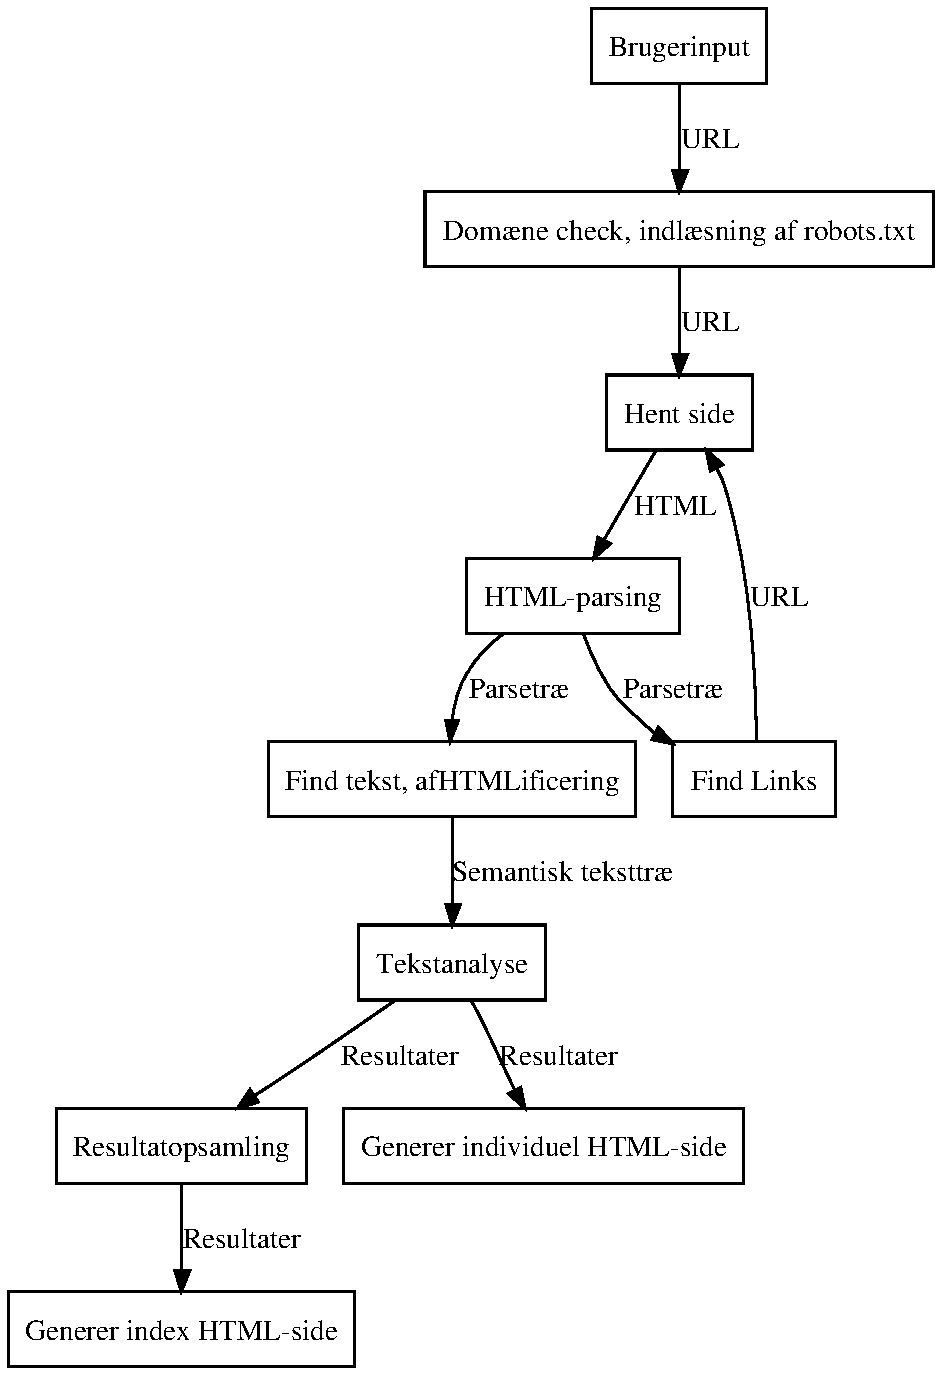
\includegraphics{designill.pdf}


\chapter{Moduler}
Vi vil nu beskrive de moduler vi har inddelt programmet i. I det
følgende henfører ``moduler'' ikke nødvendigvis til Standard ML's
moduler-feature, selvom det ikke kan afvises at dette sprogkoncept vil
blive brugt til at implementere enkelte af dem.

\section{Brugerinput}
Dette modul skal sætte en analyse i gang ud fra de parametre brugeren
angiver. Det skal også parse kommandolinjeparametrene og videregive
brugerindstillingerne til de andre moduler i programmet. Hvis
kommandolinjen er i et ugyldigt format, eller der er angivet ukendte
indstillinger, er det også dette moduls ansvar at informere brugeren
om fejlen og afslutte programmet.

\section{Indstillinger}
Da de brugerleverede indstillinger skal kunne tilgås fra vidt spredte
dele af programmet har vi fundet det bedst at lagre disse på et
centralt, løst koblet sted, i modsætning til programmets egentligt
arbejds-data, der i højere grad fører data rundt gennem tæt koblede
moduler og strenge, typestærke interfaces. Dette sikrer også at det er
let at tilføje nye indstillingsmuligheder - idet der kun skal ændres i
den kode der rent faktisk udnytter den nye indstillingsmulighed - hvor
ændringer i det primære dataflow kan resultere i en kaskade af
ændringer over det meste af programmet. Den uafhængige plads
indstillings-informationen har ville dog ikke være nær så passende til
den primære data, idet det ville gøre det sværere at kontrollere hvor
og hvornår den blev ændret, og ville svække muligheden for at
garantere den sekventielt løbende raffinering af arbejdsdata som
programmet er bygget op omkring.

\section{Domæne check, indlæsning af robots.txt}
Dette modul skal tjekke om det domæne brugeren har angivet kan tilgås
og give en fejlmeddelelse hvis det ikke er tilfældet. Hvis brugeren
har angivet det skal det undersøges om der er en
\textit{robots.txt}-fil (en standard, der gør det muligt for websider
at bede robotter om at lade være med at besøge dele af
siden) \footnote{\url{http://www.robotstxt.org/}} på serveren og hvis
det er tilfældet så skal den parses. Informationerne i
\textit{robots.txt} skal gøres tilgængeligt for \textit{Hent
  side}--modulet, så det kan se hvilke dele af websitet det må crawle.

\section{Hent Side}
Hent side modulet skal kunne hente en side fra en webserver via
HTTP-protokollen. Da vores behov er små og vi ikke har for meget tid
vil vi bruge et eksternt produceret
Http-modul\footnote{\url{http://www.diku.dk/undervisning/2000e/dat0/filer200001/K1/brevkasse.html}},
modificeret til vores behov. Det er også dette moduls job at tjekke om
\textit{robots.txt} tillader at vi må crawle siden, da dette skal tjekkes
hver gang der skal hentes en side.

\section{HTML-Parsing}
For at kunne udtrække tekst fra en HTML-side er det nødvendigt først
at parse den. Da vi ikke har været i stand til at finde en HTML-parser
skrevet i SML har vi valgt at implementere denne selv. Resultatet af
HTML-parsingen er et ordinært parsetræ som så i senere moduler bruges
til både at danne et mere højniveau-træ over teksten, og til at finde
links til andre sider som skal hentes.

Parseren er, for at lette implementationen, opdelt i to primære dele -
en lexer, der opdeler den inkommende sekvens af tegn i en liste af
leksikalske enheder uden nærmere struktur, og en egentlig parser, som
omdanner listen af de leksikale enheder til et struktureret
parsetræ. Lexeren er specificeret med en SML-signatur, men det er ikke
hensigten at denne bruges af andet end parser-modulet, og resten af
programmet vil ikke være påvirket af parsertrinnets toparts-opdeling.

De leksikale enheder produceret af lexeren vil være af tre forskellige
typer - begyndelsestags, afslutningstags og tekstelementer. De to
tag-typer vil indeholde information om navnet på det relevante tag,
samt en liste indeholdende attribut/værdi-tupler. Tekstelementer vil
indeholde information om den sekvens af tegn de repræsenterer.

Det af parseren producerede parsetræ består af knuder, repræsenterende
tags, og blade, repræsenterende tekst. En knude kan have nul eller
flere undergrene der angiver de HTML-elementer der findes mellem
start- og slut-tagget (nul undergrene kunne f.eks. være et
``\texttt{<br />}''-element), hvor hver undergren igen kan være enten
en knude eller et blad. For eksempel vil HTML-strengen
``\texttt{<strong>}\texttt{<em>}Vigtigt!\texttt{</em>} Parseren skal
fungere\texttt{</strong>}'' bestå af en knude med to undergrene -
endnu en knude og et blad indeholdende tekst. Undergrenene skal være
ordnede i samme rækkefølge som deres optræden i det oprindelige
HTML-dokument. En knude indeholder information om hvilket tag den
repræsenterer, samt eventuelle HTML-attributes tagget har.

\section{Find links}
Dette modul skal ud fra HTML-parsetræet genereret af HTML-parseren,
lave en liste af de links som linker til andre sider på samme domæne.
Det skal derefter bede om at disse sider bliver hentet, parset og
analyseret, og undersøge links på de nyhentede sider - en rekursiv
proces der løber indtil alle tilgængelige sider er blevet analyseret.

For at finde linksene skal alle \texttt{a}--tags findes --- deres
\texttt{href} attribut angiver så det link der peges på. De adresser
man finder kan være relative til den nuværende side, den absolutte
adresse til den nuværende side skal derfor kombineres med den relative
sti fra linket for at forme linkets absolutte sti. Det er dog ikke
altid den nuværende sides absolutte sti som adresser skal være
relative til, man angive en anden sti som de skal være relative til
med \texttt{base}--tagget. 

Det er ikke kun \texttt{a} der skal undersøges, hvis et HTML--dokument
benytter sig af rammer (frames), så skal deres start--adresser også
findes. Der er også andre tags der tillader at man specificerer
adresser til forklaringer ol, disse skal der også tages hån om.

På diagrammet går kun en enkelt pil fra ``Find links''-modulet til
``Hent side''-modulet. Reelt bliver denne pil fulgt for hvert eneste
fundet link som ikke allerede er blevet besøgt - resultatet bliver at
cyklussen i diagrammet fungerer som programmets primære loop der
henter og analyserer links, indtil der ikke kan findes flere indenfor
den angivne maksimaldybde.

\section{Tekstudtrækker}
Når et HTML-dokument er parset kan vi udtage teksten, det er dette
moduls job at læse parsetræet for et HTML-dokument og omdanne det til
afsnit, sætninger, overskrifter osv, som \textit{Tekstanalyse}-modulet
kan analysere. Udover at opdele teksten skal de enkelte tekstpassagers
semantiske betydning bibeholdes.

Resultatet er en datastruktur indeholdende en liste af tekstafsnit
(hvor ``afsnit'' er løst defineret og kan indeholde hvad der
oprindeligt var tabeller, eller lister, i HTML), hvert indeholdende
sætninger, og disse indeholdende ord. Hvert ord har semantisk
information fra HTML'en tilknyttet, som f.eks. information om hvorvidt
ordet er en forkortelse, eller oprindeligt har været inde i et
\texttt{em}-tag. For hvert afsnit er der også en liste over ``ekstra''
sætninger, som er den tekst der ikke umiddelbart optræder på
HTML-siden, men som alligevel er interessant - såsom \texttt{title} og
\texttt{alt}-tekst for links og billeder.

For ikke at låse programmet fuldstændig fast til HTML er dette modul
delt i to delmoduler. Det ene modul (den egentlige tekstudtrækker)
kender til selve HTML-formatet og omdanner det til en mere generisk
datastruktur der symboliserer et dokument. Denne datastruktur
indeholder information om tekstens inddeling i afsnit, overskrifter,
citater mm. Datastrukturen viderebehandles af det andet delmodul
(``sætningsifikatoren''), som udfører de beregninger der er ens for
alle dokumenter. Dette inkluderer adskillelse af ord og punktuering
(mellemrum, tegnsætning mv.) og opdeling i sætninger.  Det første
delmodul kan på denne måde let udvides så det også kan håndtere andre
dokumentformater

\section{Tekstanalyse}
Her skal de egentlige analyser foretages, modulet får teksten fra
\textit{Tekstudtrækkeren} og udfører de af brugeren valgte
tekstanalyser.

Til beregning af både lixtal og FKRT skal bruges informationer om
bl.a. antal ord og antal sætninger. Det vil resultere i dobbeltarbejde
hvis flere analyser beregner disse tal, så vi vil lave en forudgående
indsamling af informationer om teksten, der kan være relevante for
flere af analyserne. Man kan også tænke sig at der skal tilføjes nye
tekstanalyser og det vil i den forbindelse også lette arbejdet med at
implementere disse.

Output fra tekstanalysemodulet er en datastruktur der meget ligner
input, men som i stedet for semantisk information har fået tilknyttet
læsesværhedsgrad-data til de leksikale enheder (afsnit, sætninger og
ord).

\section{Generer individuelle HTML-sider}
Dette modul skal lave de HTML-filer der skal præsentere
analyseresultaterne for brugeren. Givet analyse resultaterne for en
enkelt side skal det generere en HTML side. HTML-siden vil få et
deterministisk navn baseret på HTML-filens navn og placering på
websitet, således at der kan skabes links til den genererede HTML-fil
fra analyseindekset. Til at generere HTML'en bruger vi et modul
baseret på Msp (ML Serverpages), dette er en del af Moscow ML's
standardbibliotek\footnote{\url{http://www.dina.kvl.dk/~sestoft/mosmllib/Msp.html}}.

\section{Resultatopsamling}
For hver side udregnes en sidesværhedsgrad som skal vises på
oversigtssiden for analyseresultatet. Dette modul skal gemme
sidesværhedsgrad for hver side, så der kan genereres en index fil når
analysen af alle undersiderne er afsluttet.

\section{Generer index HTML-side}
For at brugeren nemt kan få adgang til analyseresultaterne vil vi også
generere en index fil. Dette skridt er det absolut sidste der tages i
programmet, og først når alle websitets undersider er blevet
analyseret.

\chapter{Redegørelse for designets kvaliteter}
Ved at bruge dette design vil vi kunne indfri alle de uundværlige krav
stillet i kravspecifikationen. Disse krav dækker, groft sagt, at
indlæse og parse en HTML-side, finde links på den, og lave en simpel
tekstanalyse (via LIX-algoritmen) på de sider der hentes. At dette er
muligt med vores design fremgår åbenlyst af dataflow-figuren. Resten
af vores krav er baseret på udvidelse af analysefaciliteterne,
udelukkende centreret omkring de trin der kommer efter parsingen. De
kan derfor alle baseres på den grundlæggende understøttelse af parsing
og hentning (og behandlining) af HTML-filer.

Alle modulerne kan testes systematisk, måske med undtagelse af
\textit{Hent side} modulet, da testen af dette modul kræver en
forbindelse til en webserver, som vi kan være sikker på ikke ændrer
indhold. Men fordi det at hente en side er meget veldefineret vil det
sandsynligvis ikke være et problem.

Den klare opdeling i moduler som udveksler data gør det muligt at
parallelisere udviklingen, således at de enkelte moduler kan
implementeres og testes for sig selv, uden at afhænge af en færdig
implementation af de andre moduler. Hvert konceptuelt modul kan, om
ikke fuldstændigt, så til en vis grad, implementeres som en SML
modulsignatur og struktur.


\end{document}
